% Szglab4
% ===========================================================================
%
\chapter{Analízis modell kidolgozása 1}

\thispagestyle{fancy}

\section{Objektum katalógus}

\subsection{Command}
\begin{tabularx}{\linewidth}{| l | X |}
\hline
\textbf{Név} & \textbf{Leírás} \tabularnewline
\hline\hline
\endhead
ChangeDirectionQuery & Egy robottól irányváltoztatást kérő parancs. Elő tudja állítani a megfelelő \textbf{ChangeDirectionTransmit} parancsot. \tabularnewline\hline

ChangeDirectionTransmit & Az az irányváltoztató parancs, amit egy cella módosítani tud a rajta található buffokkal. Elő tudja állítani a megfelelő \textbf{ChangeDirectionExecute} parancsot. \tabularnewline\hline 

ChangeDirectionExecute & Az ugrást a \textbf{Roboton} ténylegesen végrehajtó parancs. \tabularnewline\hline

ChangeSpeedQuery & Egy robottól sebességváltoztatást kérő parancs. Elő tudja állítani a megfelelő \textbf{ChangeSpeedTransmit} parancsot. \tabularnewline\hline

ChangeSpeedTransmit & Az a sebességváltoztató parancs, amit egy cella módosítani tud a rajta található buffokkal. Elő tudja állítani a megfelelő \textbf{ChangeSpeedExecute} parancsot. \tabularnewline\hline

ChangeSpeedExecute & A sebességváltoztatást a \textbf{Roboton} ténylegesen végrehajtó parancs. \tabularnewline\hline

JumpQuery & Egy robottól ugrás kezdeményezését kérő parancs. Lekérdezi és tárolja a robot aktuális sebességét. Elő tudja állítani a megfelelő \textbf{JumpTransmit} parancsot.  \tabularnewline\hline

JumpTransmit & Az az ugróparancs, amit egy cella módosítani tud a rajta található buffokkal. Lekérdezi a cellától az ugrás kezdetét és célját, és tárolja ezeket. Elő tudja állítani a megfelelő \textbf{JumpExecute} parancsot. \tabularnewline\hline 

JumpExecute & Az ugrást a \textbf{Roboton}, a kezdő és cél cellán ténylegesen végrehajtó parancs. \tabularnewline\hline

KillExecute & Egy \textbf{Robotot} a játékból kiiktatni képes parancs. \tabularnewline\hline

TimoutExecute & Egy \textbf{Robotnak} jelzi, hogy elfogyott a rá kijelölt teljes időtartam. \tabularnewline\hline

UseOilQuery & Egy \textbf{Robotot} arra utasít, hogy helyezzen egy \textbf{Oil} buffot arra a mezőre, amelyen áll. Lekérdezi, hogy a robotnak van-e elérhető \textbf{Oil} készlete, és ezt tárolja. Elő tudja állítani a megfelelő \textbf{UseOilExecute} parancsot. \tabularnewline\hline

UseOilExecute & Egy \textbf{Oil} buffot helyez el a cellán. \tabularnewline\hline

UseStickyQuery & Egy \textbf{Robotot} arra utasít, hogy helyezzen egy \textbf{Sticky} buffot arra a mezőre, amelyen áll. Lekérdezi, hogy a robotnak van-e elérhető \textbf{Sticky} készlete, és ezt tárolja. Elő tudja állítani a megfelelő \textbf{UseStickyExecute} parancsot. \tabularnewline\hline

UseStickyExecute & Egy \textbf{Sticky} buffot helyez el a cellán. \tabularnewline\hline
\end{tabularx}

\subsection{Direction}
Tárolja egy \textbf{Robot} lehetséges mozgási irányait, és egyben a megfelelő \textbf{Cellek} lehetséges szomszédossági viszonyait.

\subsection{EmptyFieldCell}
Az \textbf{EmptyFieldCell} osztály példányai a pálya azon részeit tárolja, amelyre lépve a \textbf{Robotok} kiesnek a játékból. Az ő felelőssége a robotnak elküldeni azt a parancsot, ami ezt a hatást előidézi (\textbf{KillExecute}).
Tárolja a rajta álló robotot, illetve referenciákat a szomszédos mezőkre, amiket a megfelelő \textbf{Direction} megadásával érhetünk el. Tartalmazza ezen felül a céltól való távolságot, amelyet a nyertes meghatározására használhatunk. Az ő felelőssége annak a cellának a megkeresése, amelyre egy \textbf{Robot} ugorhat. A cellán átmenő parancsokat módosíthatja a rajta található buffokkal.

\subsection{FieldCell}
Ezen osztály példányai alkotják a pálya legnagyobb részét: minden olyan cella, amely nem a célvonal része, illetve nem a pálya szélét alkotja ilyen típusú. A \textbf{FieldCell} példányok fontos feldata, hogy a rálépő \textbf{Robotokon} érvényesítse a cellán lévő buffokat. Ezen felül a \textbf{Robotoknak} érkező parancsok egy része keresztülhalad ezeken a mezőkön, ahol a rajta található buffok ezeket a parancsokat módosíthatják. A \textbf{FieldCell} ezután a módosított parancsot
továbbítja a rajta álló \textbf{Robot} felé.
Tárolja a rajta álló robotot, illetve referenciákat a szomszédos mezőkre, amiket a megfelelő \textbf{Direction} megadásával érhetünk el. Tartalmazza ezen felül a céltól való távolságot, amelyet a nyertes meghatározására használhatunk. Az ő felelőssége annak a cellának a megkeresése, amelyre egy \textbf{Robot} ugorhat. A cellán átmenő parancsokat módosíthatja a rajta található buffokkal.

\subsection{FinishLineFieldCell}
A \textbf{FinishLineFieldCell} osztály példányainak felelősségei megegyeznek a \textbf{FieldCell} osztály példányainak felelősségeivel, azzal a különbséggel, hogy ezek a cellák jelzik egy körnek a végét.

\subsection{Inventory}
Buffok tárolására alkalmas, nyílvántartja a benne található buffok számát, és csak akkor engedi azokat használni, ha legalább egyet tartalmaz.

\subsection{Oil}
Egy olyan buff, aminek hatására a \textbf{Fieldre} lépő \textbf{Robotok} sebessége megfelelződik.

\subsection{Result}
Egy parancs lefutásának eredményét tárolja.

\subsection{Robot}
A \textbf{Robot} osztály példányai egy-egy pályán mozgó robotot tárolnak. Tárolja a saját sebességét, illetve azt a cellát, amin pillanatnyilag áll. Ezen felül rendelkeznek \textbf{Inventorykkal}, amelyben \textbf{Stickyt} vagy \textbf{Oilt} tárolnak. Ezeket le tudják helyezni arra a cellára, amelyen állnak.

\subsection{Speed}
Egy \textbf{Robot} sebességét reprezentálja.

\subsection{Sticky}
Egy olyan buff, ami képes a \textbf{JumpExecute} parancs olyan módosítására, amely megakadályozza azt, hogy ez a parancs megváltoztassa egy \textbf{Robot} sebességét.


\begin{figure}[h]
\begin{center}
%\includegraphics[width=17cm]{chapters/chapter03/example.pdf}
\caption{x}
\label{fig:example1}
\end{center}
\end{figure}


\section{Osztályok leírása}

\subsection{AgentElement <<Interface>>}
\begin{itemize}

\item Felelősség\\
Ez az osztály képes AgentVisitorok és AgentCommandek fogadására. 

\item Ősosztályok\\
Nincs

\item Interfészek\\
Nincs

\item Attribútumok\\
Nincs

\item Metódusok\\

\begin{itemize}
    \item void accept(visitor: AgentVisitor): ez a metódus képes az AgentVisitor fogadására
    \item void accept(visitor: AgentCommand): ez a metódus képes az AgentCommand fogadására
\end{itemize}

\end{itemize}

\subsection{AgentVisitor <<Interface>>}
\begin{itemize}

\item Felelősség\\
Az Agent absztrakt osztály leszármazott osztályainak meglátogatására képes.

\item Ősosztályok\\
Nincs

\item Interfészek\\
Nincs

\item Attribútumok\\
Nincs

\item Metódusok\\

\begin{itemize}
    \item void visit(element: Robot): meglátogat egy robotot
\end{itemize}

\end{itemize}


\subsection{Agent <<Abstract>>}
\begin{itemize}

\item Felelősség\\
A pályán lévő összes ágens közös viselkedését valósítja meg. 

\item Ősosztályok\\
Nincs

\item Interfészek\\
AgentElement

\item Attribútumok\\
\begin{itemize}
    \item field: Field
    \item speed: Speed
    \item isDead: bool
    \item isOutOfTime: bool
    \item currentLeft: int
\end{itemize}

\item Metódusok\\

\begin{itemize}
    \item Speed getSpeed(void): visszaadja az Agent sebességét
    \item void setSpeed(speed: Speed): beállítja az Agent sebességét
    \item Field getField(void): visszaadja a mezőt, ahol az Agent áll
    \item void setField(field: Field): beállítja, hogy melyik mezőn áll az Agent
    \item bool isDead(void): megmondja, hogy Agent halott-e
    \item void kill(void): megöli az Agentet
    \item bool isOutOfTime(void): megmondja, hogy az Agentnek van-e még ideje lépni
    \item void getLap(void): megmondja, hogy hányadik körben van az Agent
    \item void incrementLap(void): növeli a kör számlálóját
\end{itemize}

\end{itemize}

\subsection{Robot}
\begin{itemize}

\item Felelősség\\
A pályán elhelyezkedő egyik Agent típus.

\item Ősosztályok\\
Agent

\item Interfészek\\
(Agent) - AgentElement

\item Attribútumok\\
\begin{itemize}
    \item stickyInventory: Inventory<Sticky>
    \item oilInventory: Inventory<Oil>
    \item buffs: Buff[]
\end{itemize}

\item Metódusok\\

\begin{itemize}
    \item bool useSticky(void): használja az Inventory<Sticky>-ben tárolt Stickyt (ragacsot)
    \item bool useOil(void): használja az Inventory<Oil>-ben tárolt Oilt (ragacsot)
    \item void addSticky(void): hozzáad egy Stickyt az Inventory<Sticky>-hez.
    \item void addOil(void): hozzáad egy Oilt az Inventory<Oil>-hez.
\end{itemize}

\end{itemize}

\subsection{Inventory}
\begin{itemize}

\item Felelősség\\
Generikus tárolós, mely képes a típusának megfelelő elemeket tenni magába, illetve használni őket.

\item Ősosztályok\\
Nincs

\item Interfészek\\
Nincs

\item Attribútumok\\
\begin{itemize}
    \item buffs: T[]
\end{itemize}

\item Metódusok\\

\begin{itemize}
    \item void addItem(item: T): hozzáad egy T típusú itemet az Inventory<T>-hez.
    \item bool useItem(void): használja az Inventory<T>-ben tárolt itemet, amennyiben nem üres igazzal tér vissza, különben hamis.
\end{itemize}

\end{itemize}

\subsection{Buff <<Abstract>>}
\begin{itemize}

\item Felelősség\\
Az összes releváns visitor implementálása. Interface collection. Commandokat és Agenteket is tud módosítani.

\item Ősosztályok\\
Nincs

\item Interfészek\\
FieldCommandVisitor\\
AgentCommandVisitor\\
AgentVisitor\\

\item Attribútumok\\
Nincs

\item Metódusok\\
Nincs

\end{itemize}

\subsection{FieldElement <<Interface>>}
\begin{itemize}

\item Felelősség\\


\item Ősosztályok\\
Nincs

\item Interfészek\\
Nincs

\item Attribútumok\\
\begin{itemize}
    \item buffs: T[]
\end{itemize}

\item Metódusok\\

\begin{itemize}
    \item void addItem(item: T): hozzáad egy T típusú itemet az Inventory<T>-hez.
    \item bool useItem(void): használja az Inventory<T>-ben tárolt itemet, amennyiben nem üres igazzal tér vissza, különben hamis.
\end{itemize}

\end{itemize}

\subsection{FieldElement <<Interface>>}
\begin{itemize}

\item Felelősség\\
Ez az osztály képes FieldVisitorok és FieldCommandek fogadására. 

\item Ősosztályok\\
Nincs

\item Interfészek\\
Nincs

\item Attribútumok\\
Nincs

\item Metódusok\\

\begin{itemize}
    \item void accept(visitor: FieldVisitor): ez a metódus képes az FieldVisitor fogadására
    \item void accept(visitor: FieldCommand): ez a metódus képes az FieldCommand fogadására
\end{itemize}

\end{itemize}

\subsection{FieldVisitor <<Interface>>}
\begin{itemize}

\item Felelősség\\
Az Field absztrakt osztály leszármazott osztályainak meglátogatására képes.

\item Ősosztályok\\
Nincs

\item Interfészek\\
Nincs

\item Attribútumok\\
Nincs

\item Metódusok\\

\begin{itemize}
    \item void visit(element: FieldCell): meglátogat egy FieldCell objektumot
    \item void visit(element: EmptyFieldCell): meglátogat egy EmptyFieldCell objektumot
    \item void visit(element: FinishFieldCell): meglátogat egy FinishFieldCell objektumot
\end{itemize}

\end{itemize}

\subsection{Field <<Abstract>>}
\begin{itemize}

\item Felelősség\\
A pályán lévő mezők viselkedését valósítja meg.

\item Ősosztályok\\
Nincs

\item Interfészek\\
Nincs

\item Attribútumok\\
    \begin{itemize}
            \item agent: Agent
            \item distanceFromGoal: int 
            \item buffs: Buff[]
            \item neighbours: Map<Direction, Field>
    \end{itemize}

\item Metódusok\\

\begin{itemize}
    \item void addNeighbour(direction: Direction, field: Field): hozzáadja a mezőhöz a megfelelő szomszédot a megfelelő irányban.
    \item void onEnter(agent: Agent): beállítja az Agent-nek önmagát, beállítja a saját agent attribútumát a rálépő Agent-re.
    \item void onExit(void): elfelejti az agentet, aki rajta állt. Kitörli az agentből önmagát.
    \item int getDistanceFromGoal(void): megmondja, hogy az mező hány mezőre van a céltól.
    \item void placeBuff(buff: Buff): a paraméterben megadott buffot a mezőre teszi
    \item Displacement getDisplacement(speed: Speed): kiszámolja, hogy adott sebességgel melyik másik mezőre lehet ugrani.
\end{itemize}

\end{itemize}

\subsection{Displacement}
\begin{itemize}

\item Felelősség\\
Az elmozdulást kezelő osztály, mely a kezdeti és végpont mezőket tudja.

\item Ősosztályok\\
Nincs

\item Interfészek\\
Nincs

\item Attribútumok\\
    \begin{itemize}
            \item start: Field
            \item goal: Field
    \end{itemize}

\item Metódusok\\

\begin{itemize}
    \item Field getStart(void): visszaadja a kezdeti mezőt
    \item Field getGoal(void): visszaadja az érkezési mezőt
\end{itemize}

\end{itemize}

\subsection{EmptyFieldCell}
\begin{itemize}

\item Felelősség\\
A pálya szélén lévő mezők.

\item Ősosztályok\\
Field

\item Interfészek\\
(Field) - FieldElement

\item Attribútumok\\
Nincs

\item Metódusok\\
Nincs

\end{itemize}


\subsection{FieldCell}
\begin{itemize}

\item Felelősség\\
Minden, ami nem pálya széle illetve nem célmező.

\item Ősosztályok\\
Field

\item Interfészek\\
(Field) - FieldElement

\item Attribútumok\\
Nincs

\item Metódusok\\
Nincs

\end{itemize}


\subsection{FinishLineFieldCell}
\begin{itemize}

\item Felelősség\\
A célt jelző mezőtípus.

\item Ősosztályok\\
Field

\item Interfészek\\
(Field) - FieldElement

\item Attribútumok\\
Nincs

\item Metódusok\\
Nincs

\end{itemize}

\subsection{Command <<Abstract>}
\begin{itemize}

\item Felelősség\\
Az összes parancs jellemző közös viselkedés megvalósítója.

\item Ősosztályok\\
Nincs

\item Interfészek\\
Nincs

\item Attribútumok\\
    \begin{itemize}
            \item canExecute: bool
    \end{itemize}

\item Metódusok\\

\begin{itemize}
    \item bool canExecute(void): igazzal tér vissza, ha a parancs végrehajtható
    \item bool setExecutable(canExecute: bool): beállítja, hogy futtatható-e a parancs
\end{itemize}

\end{itemize}

\subsection{AgentCommand <<Abstract>}
\begin{itemize}

\item Felelősség\\
Az Agentre vonatkozó parancsok, közös viselkedést megvalósító osztály.

\item Ősosztályok\\
Nincs

\item Interfészek\\
AgentVisitor

\item Attribútumok\\
Nincs

\item Metódusok\\

\begin{itemize}
    \item FieldCommand getFieldCommand(void): amennyiben a parancsláncban szükeséges egy mezőnek átadni a parancsot, ezt állítja elő.
    \item void accept(element: AgentCommandVisitor): a buffok ezen keresztül tudják módosítani a parancsokat.
\end{itemize}

\end{itemize}

\subsection{FieldCommand <<Abstract>}
\begin{itemize}

\item Felelősség\\
Az Fieldre vonatkozó parancsok, közös viselkedést megvalósító osztály.

\item Ősosztályok\\
Nincs

\item Interfészek\\
FieldVisitor

\item Attribútumok\\
Nincs

\item Metódusok\\

\begin{itemize}
    \item FieldCommand getFieldCommand(void): amennyiben a parancsláncban szükeséges egy mezőnek átadni a parancsot, ezt állítja elő.
    \item void accept(element: FieldCommandVisitor): a buffok ezen keresztül tudják módosítani a parancsokat.
\end{itemize}

\end{itemize}



\clearpage

\section{Statikus struktúra diagramok}

\begin{figure}[h]
\begin{center}
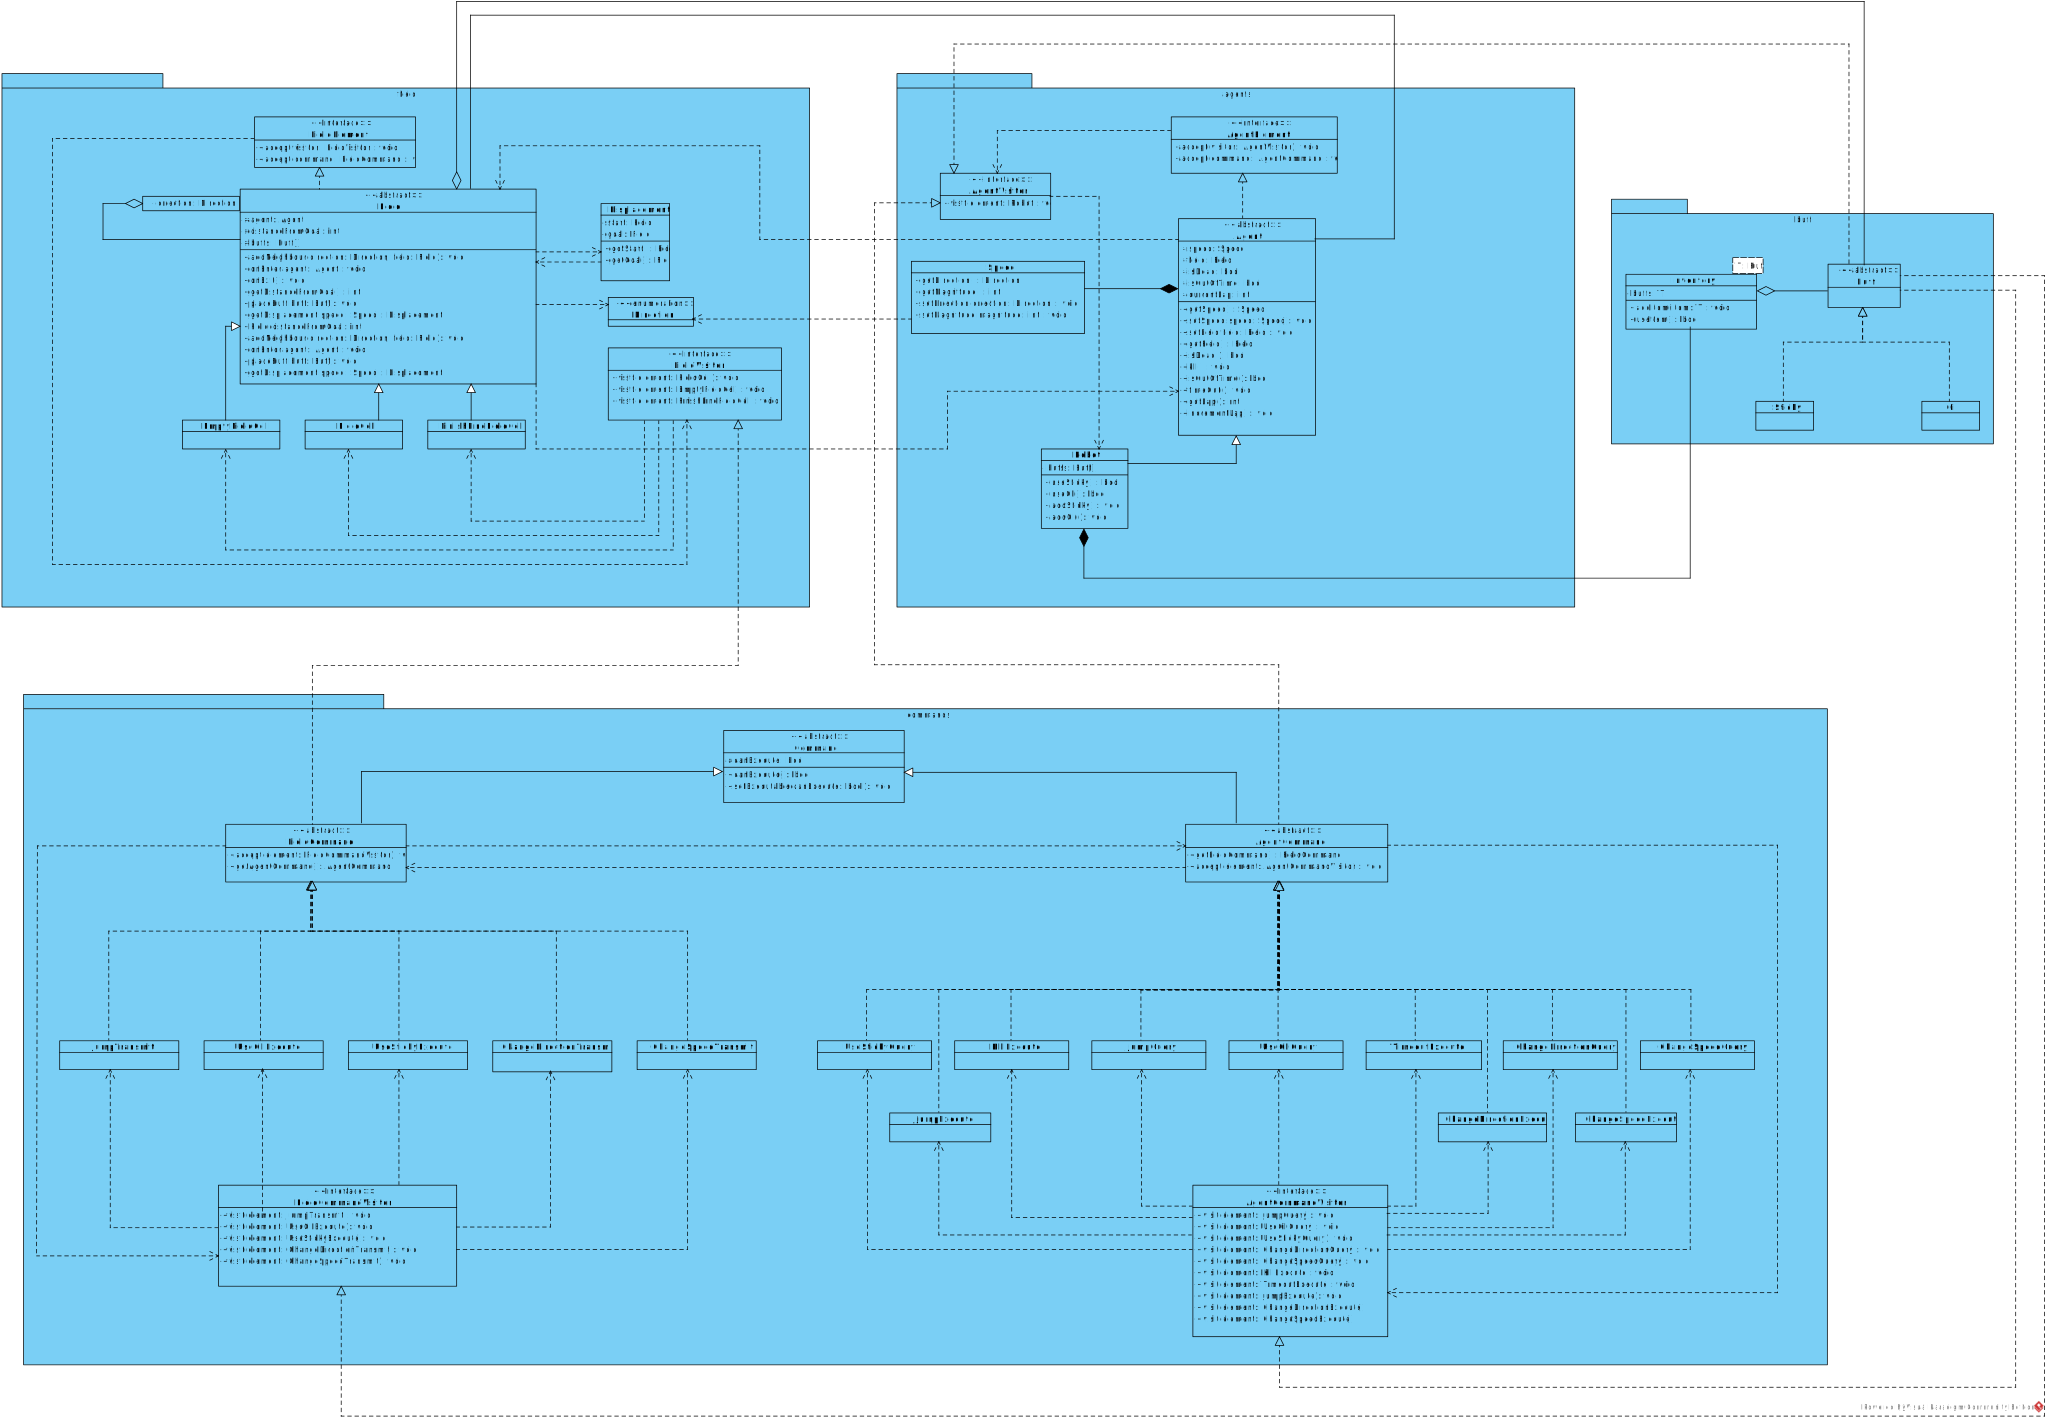
\includegraphics[width=\linewidth]{chapters/chapter03/ClassMain.pdf}
\caption{A teljes osztálydiagram}
\label{A teljes osztálydiagram}
\end{center}
\end{figure}

\begin{figure}[h]
\begin{center}
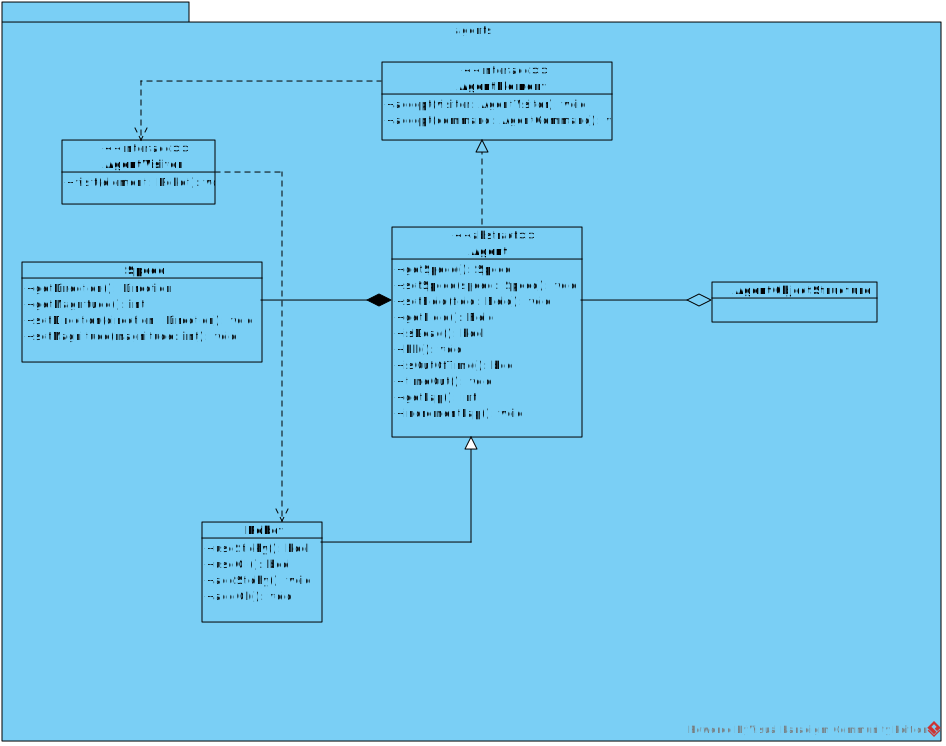
\includegraphics[width=\linewidth]{chapters/chapter03/ClassAgents.pdf}
\caption{Agents package osztálydiagram}
\label{Agents package osztálydiagram}
\end{center}
\end{figure}

\begin{figure}[h]
\begin{center}
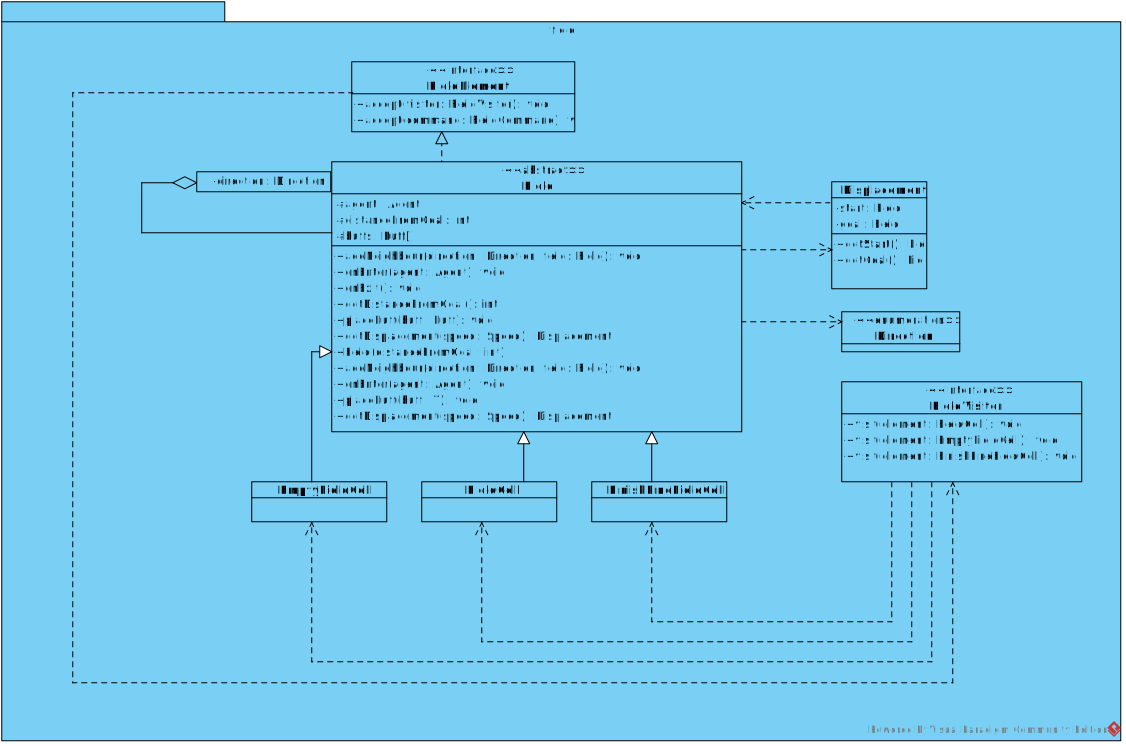
\includegraphics[width=\linewidth]{chapters/chapter03/ClassField.pdf}
\caption{Field package osztálydiagram}
\label{Field package osztálydiagram}
\end{center}
\end{figure}

\clearpage

\begin{figure}[h]
\begin{center}
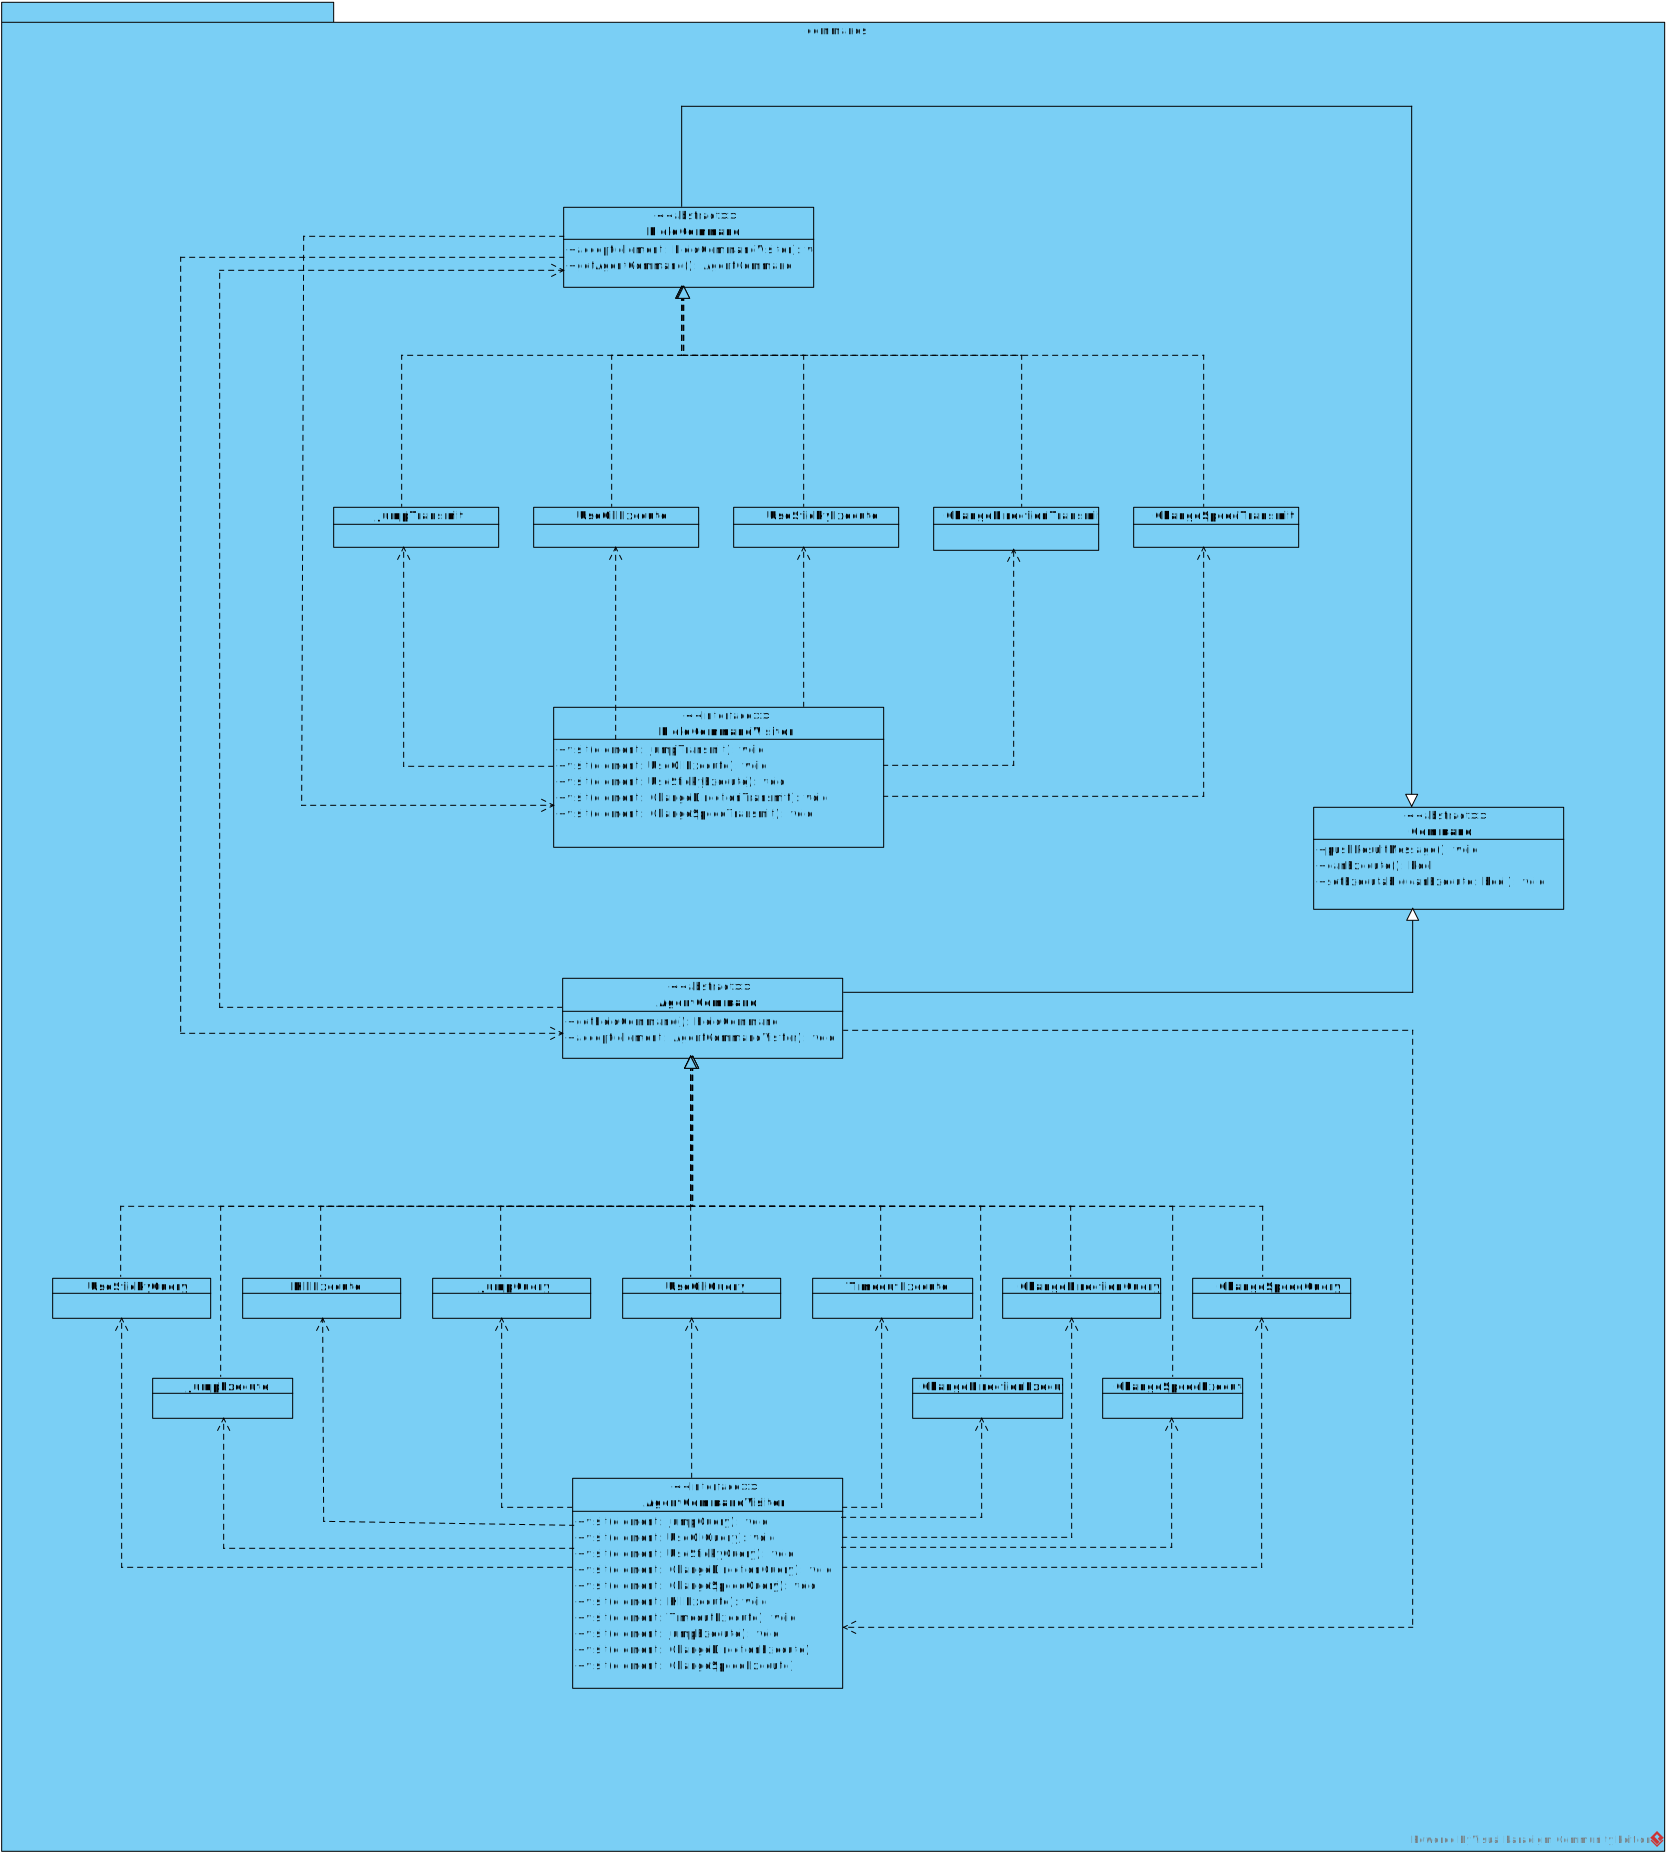
\includegraphics[width=\linewidth]{chapters/chapter03/ClassCommands.pdf}
\caption{Commands package osztálydiagram}
\label{Commands package osztálydiagram}
\end{center}
\end{figure}


\begin{figure}[h]
\begin{center}
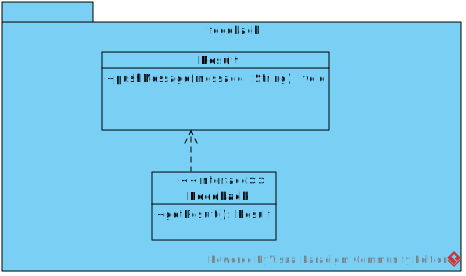
\includegraphics[width=\linewidth]{chapters/chapter03/ClassFeedback.pdf}
\caption{Feedback package osztálydiagram}
\label{Feedback package osztálydiagram}
\end{center}
\end{figure}


\begin{figure}[h]
\begin{center}
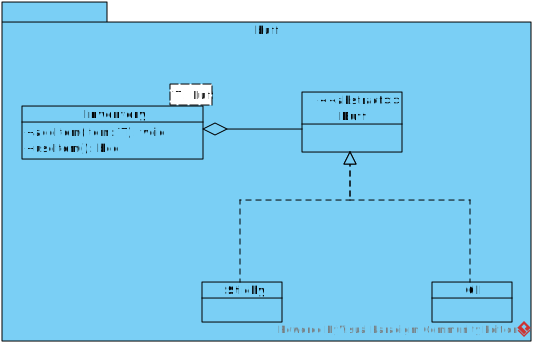
\includegraphics[width=\linewidth]{chapters/chapter03/ClassBuff.pdf}
\caption{Buff package osztálydiagram}
\label{Buff package osztálydiagram}
\end{center}
\end{figure}


\begin{figure}[h]
\begin{center}
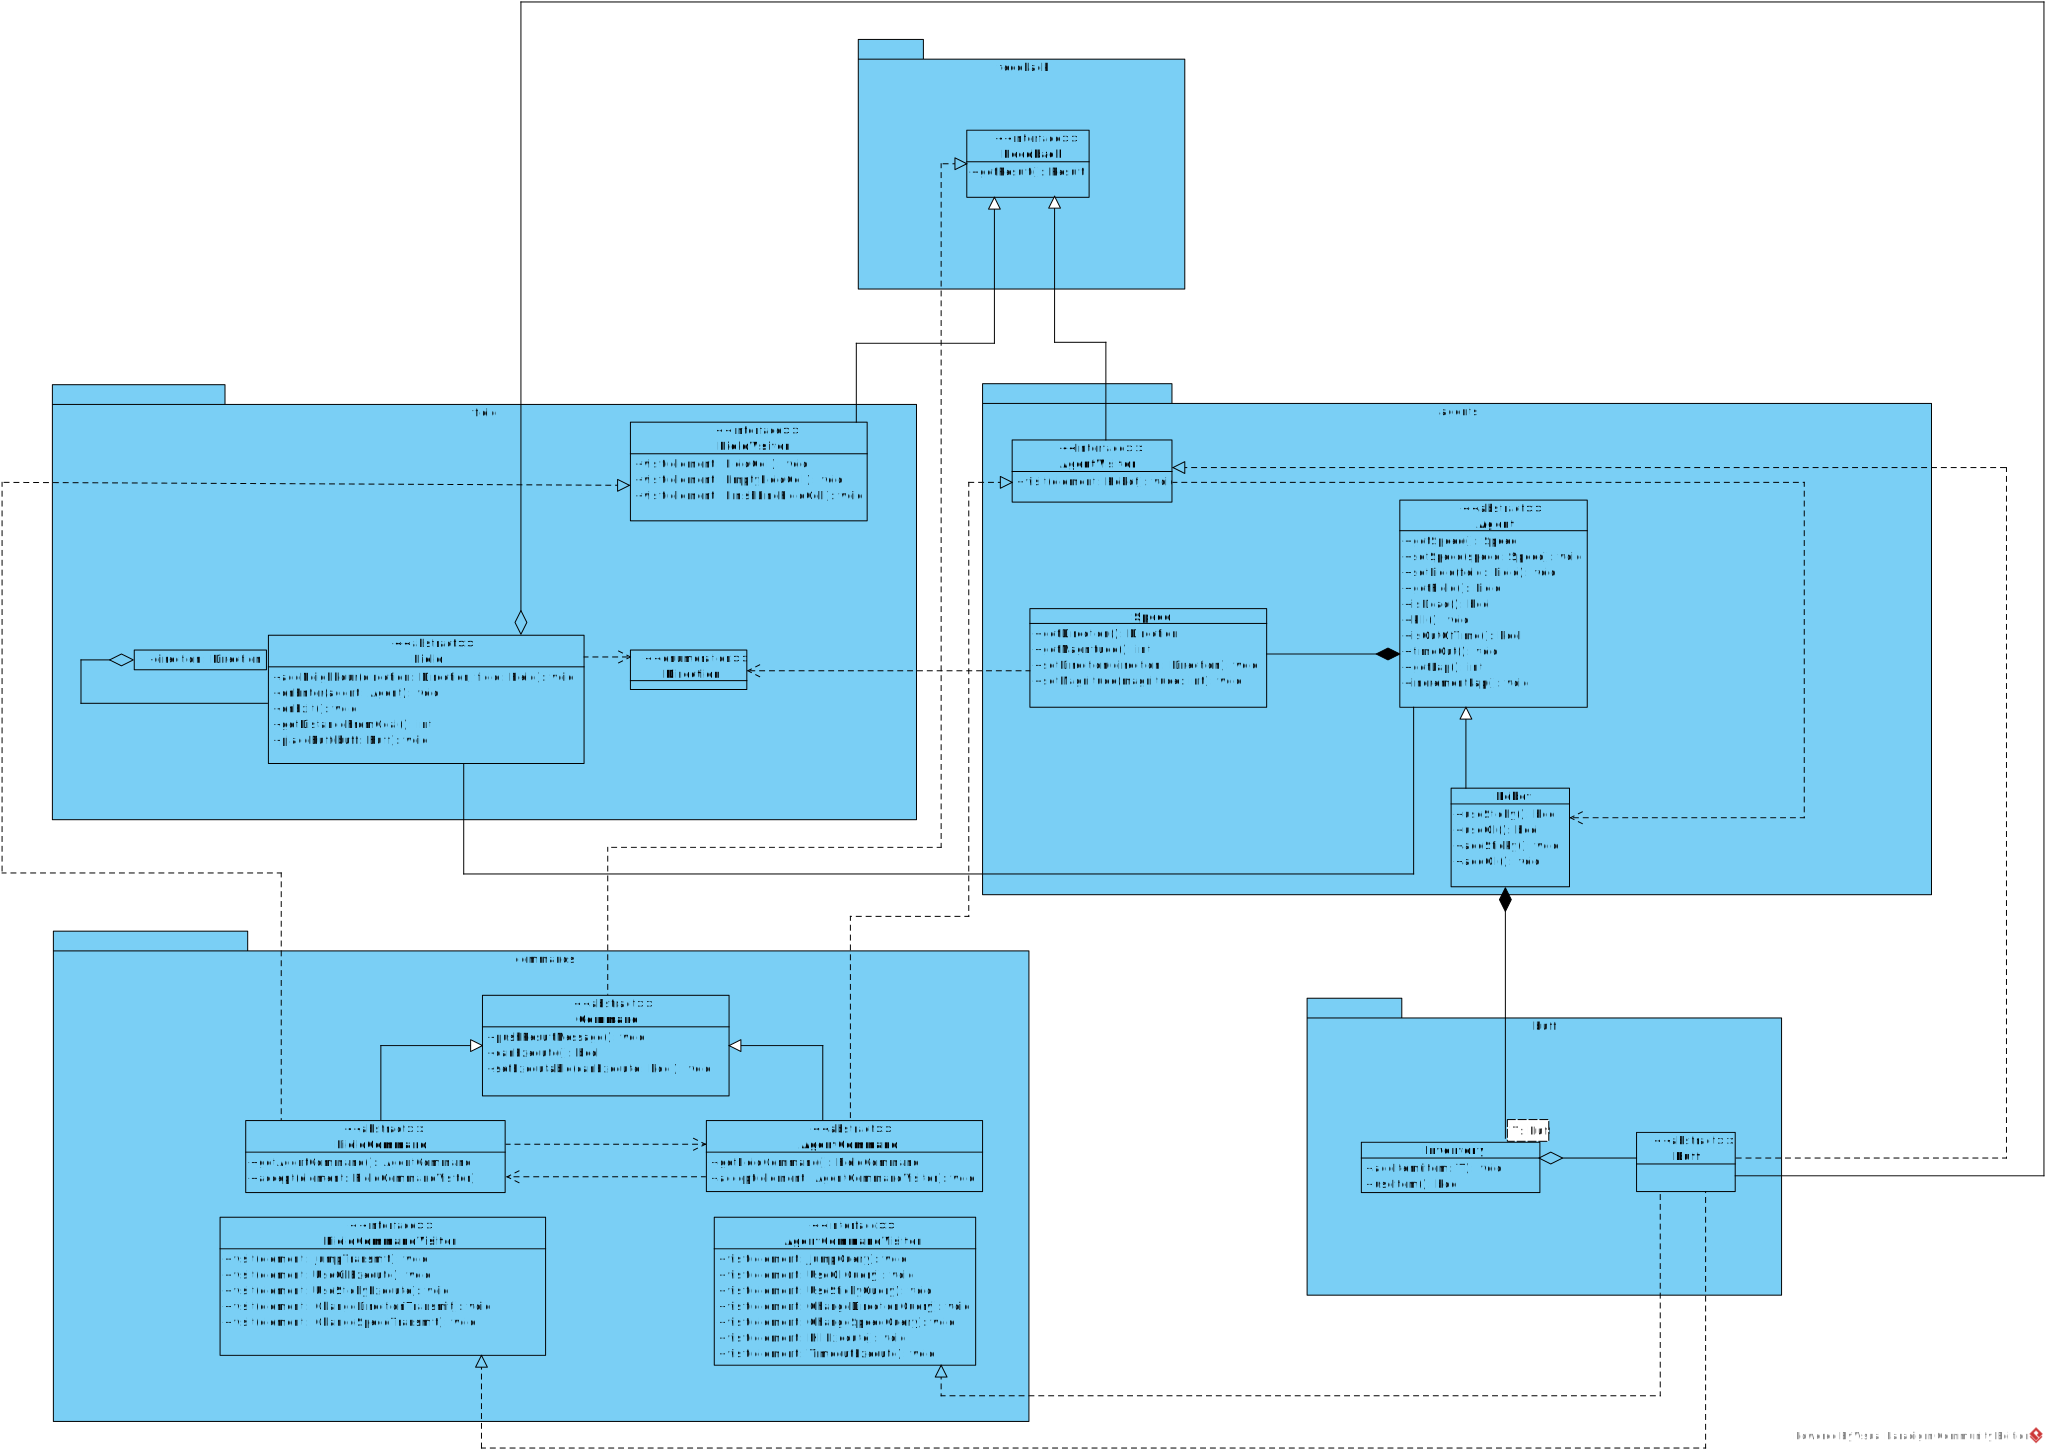
\includegraphics[width=\linewidth]{chapters/chapter03/ClassInterpackage.pdf}
\caption{Packagek közti függőségek osztálydiagramja}
\label{Packagek közti függőségek osztálydiagramja}
\end{center}
\end{figure}

\clearpage

\section{Szekvencia diagramok}

\begin{figure}[h]
	\begin{center}
		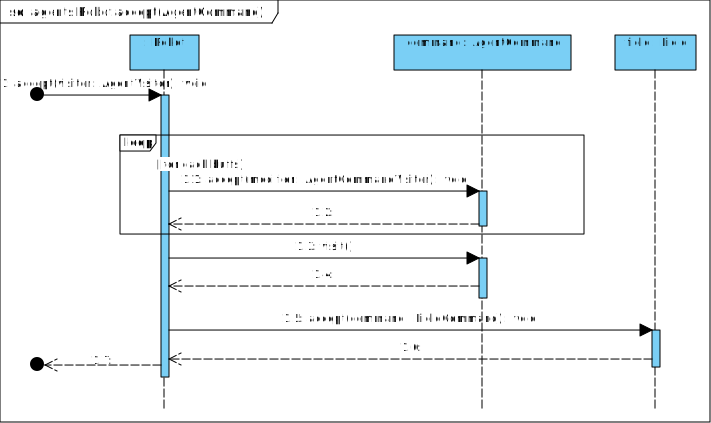
\includegraphics[width=\textwidth]{chapters/chapter03/agentsRobotacceptAgentCommand.pdf}
		\caption{Robot utasítást fogad}
		\label{fig:agents.Robot.accept}
	\end{center}
\end{figure}

\begin{figure}[h]
	\begin{center}
		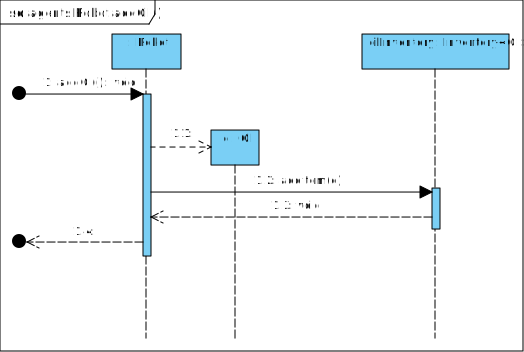
\includegraphics[width=\textwidth]{chapters/chapter03/agentsRobotaddOil.pdf}
		\caption{Robot felvesz a készletébe egy olajfoltot}
		\label{fig:agents.Robot.addOil}
	\end{center}
\end{figure}

\begin{figure}[h]
	\begin{center}
		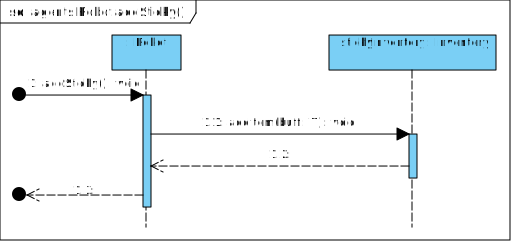
\includegraphics[width=\textwidth]{chapters/chapter03/agentsRobotaddSticky.pdf}
		\caption{Robot felvesz a készletébe egy ragacsfoltot}
		\label{fig:agents.Robot.addSticky}
	\end{center}
\end{figure}

\begin{figure}[h]
	\begin{center}
		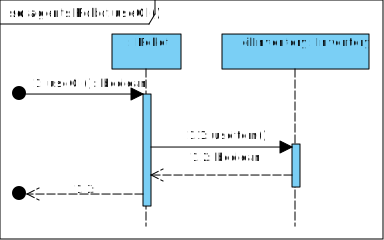
\includegraphics[width=\textwidth]{chapters/chapter03/agentsRobotuseOil.pdf}
		\caption{Robot felhasználja a készletében lévő olajfoltot ha van}
		\label{fig:agents.Robot.useOil}
	\end{center}
\end{figure}

\begin{figure}[h]
	\begin{center}
		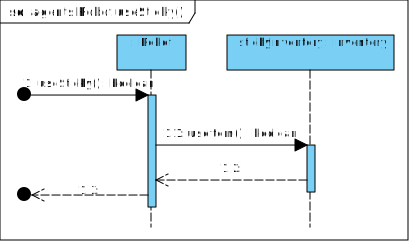
\includegraphics[width=\textwidth]{chapters/chapter03/agentsRobotuseSticky.pdf}
		\caption{Robot felhasználja a készletében lévő ragacsfoltot ha van}
		\label{fig:agents.Robot.useSticky}
	\end{center}
\end{figure}

\begin{figure}[h]
	\begin{center}
		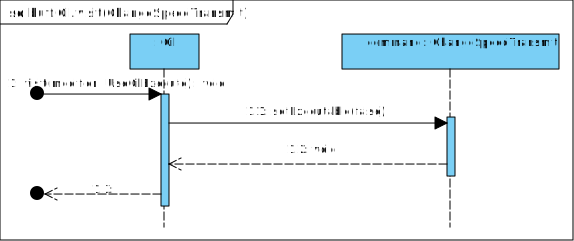
\includegraphics[width=\textwidth]{chapters/chapter03/buffOilvisitChangeSpeedTransmit.pdf}
		\caption{Olajfolt megakadályozza a sebesség nagyságának változtatását}
		\label{fig:buff.Oil.visit}
	\end{center}
\end{figure}

\begin{figure}[h]
	\begin{center}
		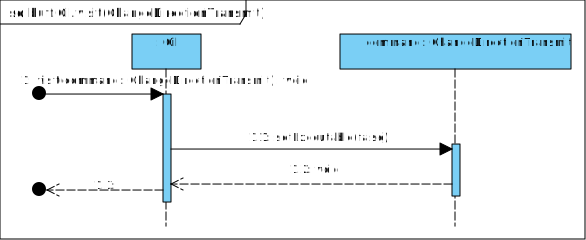
\includegraphics[width=\textwidth]{chapters/chapter03/buffOilvisitChangeDirectionTransmit.pdf}
		\caption{Olajfolt megakadályozza a sebesség irányának megváltoztatását}
		\label{fig:buff.Oil.visit2}
	\end{center}
\end{figure}

\begin{figure}[h]
	\begin{center}
		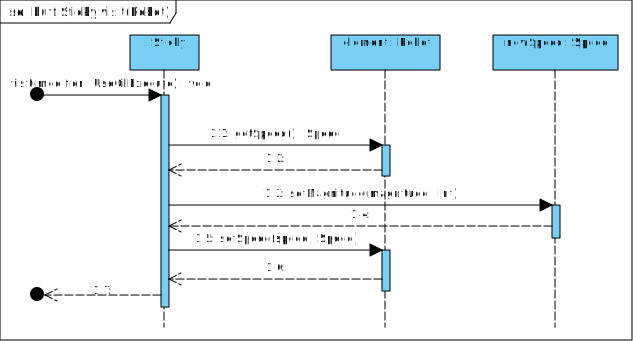
\includegraphics[width=\textwidth]{chapters/chapter03/buffStickyvisitRobot.pdf}
		\caption{Olajfolt megakadályozza a sebességváltoztatást}
		\label{fig:buff.Sticky.visit}
	\end{center}
\end{figure}

\begin{figure}[h]
	\begin{center}
		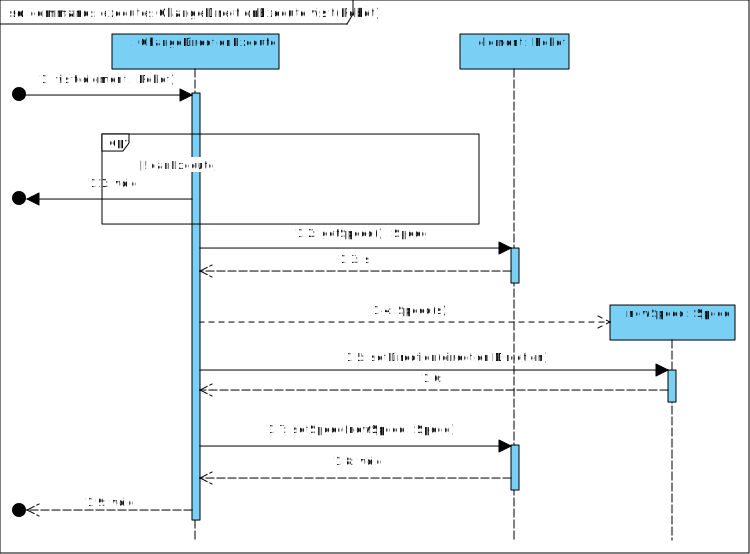
\includegraphics[width=\textwidth]{chapters/chapter03/commandsexecutesChangeDirectionExecutevisitRobot.pdf}
		\caption{Robot irányváltoztatásának végrehajtása}
		\label{fig:command.executes.ChangeDirectionExecute.visit}
	\end{center}
\end{figure}

\begin{figure}[h]
	\begin{center}
		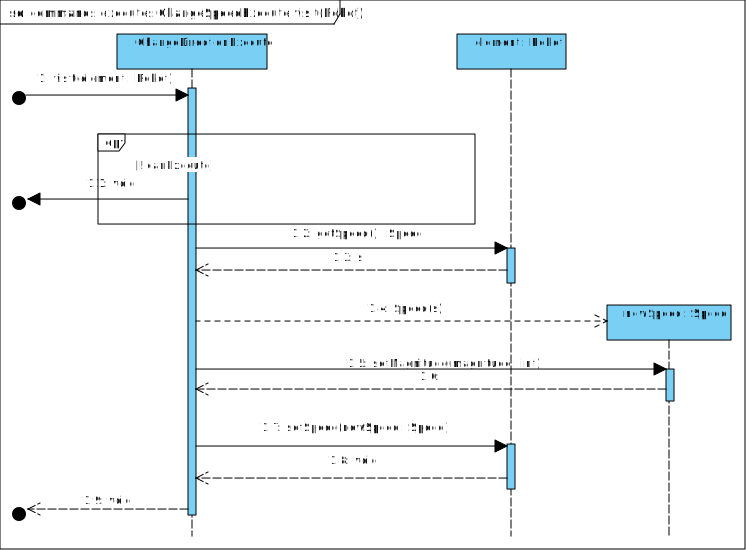
\includegraphics[width=\textwidth]{chapters/chapter03/commandsexecutesChangeSpeedExecutevisitRobot.pdf}
		\caption{Robot sebességnagyságának megváltoztatása}
		\label{fig:command.executes.ChangeSpeedExecute.visit}
	\end{center}
\end{figure}

\begin{figure}[h]
	\begin{center}
		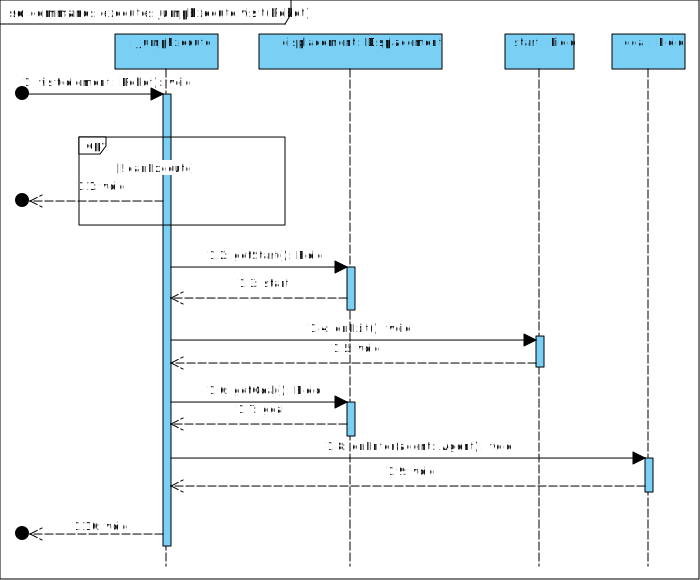
\includegraphics[width=\textwidth]{chapters/chapter03/commandsexecutesJumpExecutevisitRobot.pdf}
		\caption{Robot ugrásának végrehajtása}
		\label{fig:command.executes.JumpExecute.visit}
	\end{center}
\end{figure}

\begin{figure}[h]
	\begin{center}
		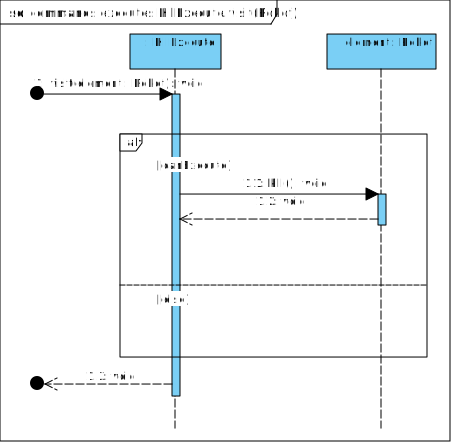
\includegraphics[width=\textwidth]{chapters/chapter03/commandsexecutesKillExecutevisitRobot.pdf}
		\caption{Robot megölésének végrehajtása}
		\label{fig:command.executes.KillExecute.visit}
	\end{center}
\end{figure}

\begin{figure}[h]
	\begin{center}
		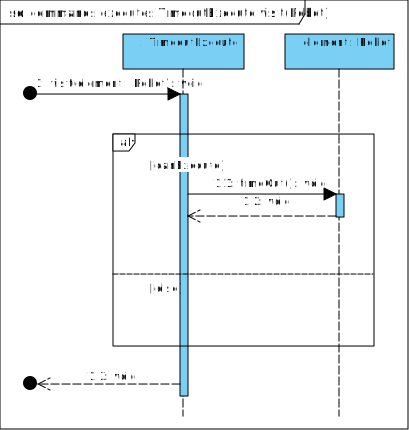
\includegraphics[width=\textwidth]{chapters/chapter03/commandsexecutesTimeoutExecutevisitRobot.pdf}
		\caption{Robot idő lejártának végrehajtása}
		\label{fig:command.executes.TimeoutExecute.visit}
	\end{center}
\end{figure}

\begin{figure}[h]
	\begin{center}
		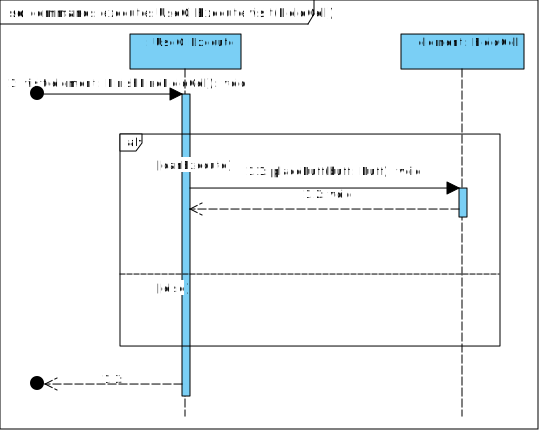
\includegraphics[width=\textwidth]{chapters/chapter03/commandsexecutesUseOilExecutevisitFieldCell.pdf}
		\caption{Robot lehelyezi az Olaj foltot a mezőre}
		\label{fig:command.executes.UseOilExecute.visit}
	\end{center}
\end{figure}

\begin{figure}[h]
	\begin{center}
		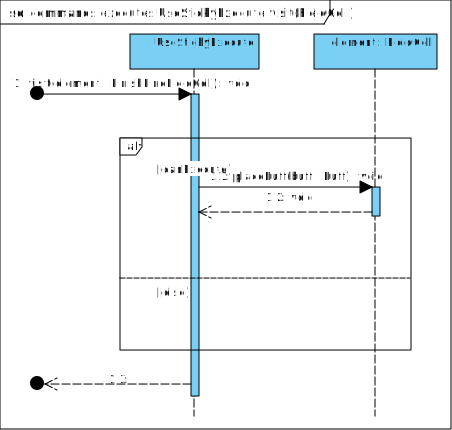
\includegraphics[width=\textwidth]{chapters/chapter03/commandsexecutesUseStickyExecutevisitFieldCell.pdf}
		\caption{Robot lehelyezi a Ragacs foltot a mezőre}
		\label{fig:command.executes.UseStickyExecute.visit}
	\end{center}
\end{figure}

\clearpage

\begin{figure}[h]
	\begin{center}
		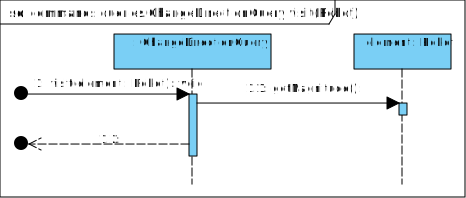
\includegraphics[width=\textwidth]{chapters/chapter03/commandsqueriesChangeDirectionQueryvisitRobot.pdf}
		\caption{Robot irányváltásra való felkérése}
		\label{fig:command.executes.ChangeDirectionQuery.visit}
	\end{center}
\end{figure}

\begin{figure}[h]
	\begin{center}
		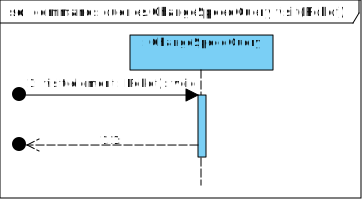
\includegraphics[width=\textwidth]{chapters/chapter03/commandsqueriesChangeSpeedQueryvisitRobot.pdf}
		\caption{Robot sebesség nagyságának megváltoztatására való felkérése}
		\label{fig:command.executes.ChangeSpeedQuery.visit}
	\end{center}
\end{figure}

\begin{figure}[h]
	\begin{center}
		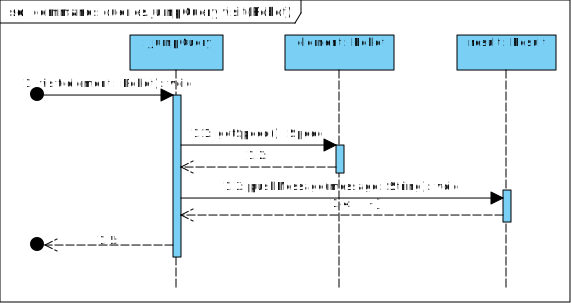
\includegraphics[width=\textwidth]{chapters/chapter03/commandsqueriesJumpQueryvisitRobot.pdf}
		\caption{Robot ugrásra azaz helyzetmódosításra való felkérése}
		\label{fig:command.executes.JumpQuery.visit}
	\end{center}
\end{figure}

\begin{figure}[h]
	\begin{center}
		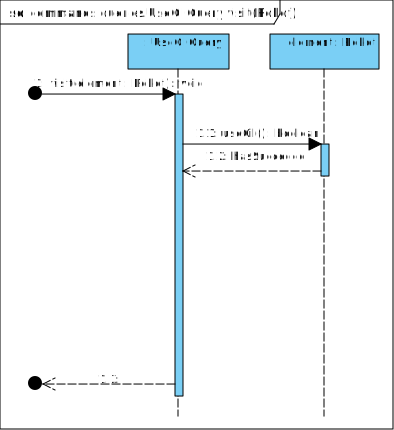
\includegraphics[width=\textwidth]{chapters/chapter03/commandsqueriesUseOilQueryvisitRobot.pdf}
		\caption{Robotot Olaj lehelyezésére való felkérése}
		\label{fig:command.executes.UseOilQuery.visit}
	\end{center}
\end{figure}

\begin{figure}[h]
	\begin{center}
		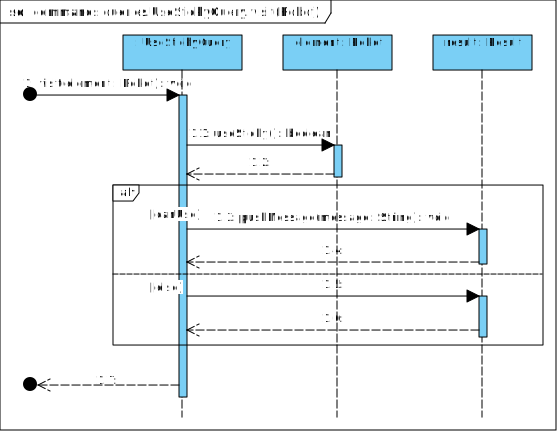
\includegraphics[width=\textwidth]{chapters/chapter03/commandsqueriesUseStickyQueryvisitRobot.pdf}
		\caption{Robotot Ragacs lehelyezésére való felkérése}
		\label{fig:command.executes.UseStickyQuery.visit}
	\end{center}
\end{figure}

\begin{figure}[h]
	\begin{center}
		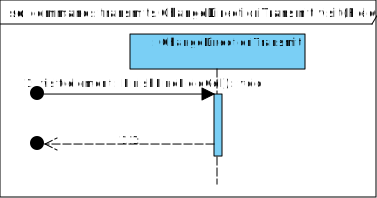
\includegraphics[width=\textwidth]{chapters/chapter03/commandstransmitsChangeDirectionTransmitvisitFieldCell.pdf}
		\caption{Irányváltásra vonatkozó kérés átvitele}
		\label{fig:command.executes.ChangeDirectionTransmit.visit}
	\end{center}
\end{figure}

\begin{figure}[h]
	\begin{center}
		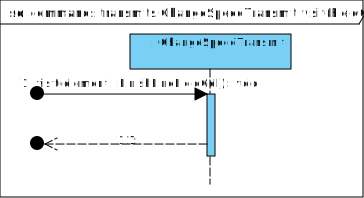
\includegraphics[width=\textwidth]{chapters/chapter03/commandstransmitsChangeSpeedTransmitvisitFieldCell.pdf}
		\caption{Szebességnagyság változtatásra vonatkozó kérés átvitele}
		\label{fig:command.executes.ChangeSpeedTransmit.visit}
	\end{center}
\end{figure}

\begin{figure}[h]
	\begin{center}
		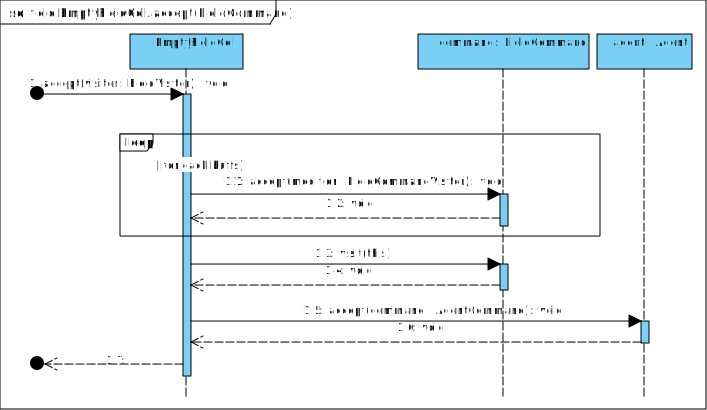
\includegraphics[width=\textwidth]{chapters/chapter03/fieldEmptyFieldCellacceptFieldCommand.pdf}
		\caption{Üres pályamező utasításfeldolgozása}
		\label{fig:field.EmptyFieldCell.accept}
	\end{center}
\end{figure}

\begin{figure}[h]
	\begin{center}
		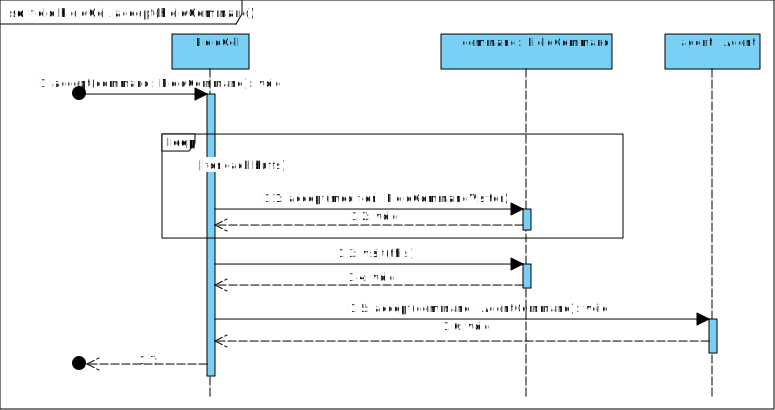
\includegraphics[width=\textwidth]{chapters/chapter03/fieldFieldCellacceptFieldCommand.pdf}
		\caption{Pályamező utasításfeldolgozása}
		\label{fig:field.FieldCell.accept}
	\end{center}
\end{figure}

\begin{figure}[h]
	\begin{center}
		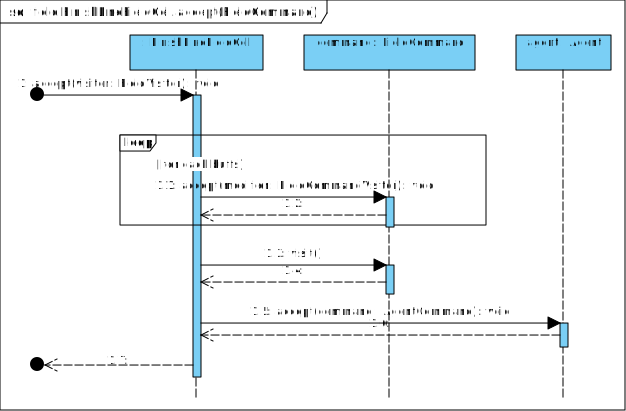
\includegraphics[width=\textwidth]{chapters/chapter03/fieldFinishLineFieldCellacceptFieldCommand.pdf}
		\caption{Start/célvonal pályamező utasításfeldolgozása}
		\label{fig:field.FinishLineFieldCell.accept}
	\end{center}
\end{figure}

\clearpage

\section{State-chartok}
\comment{Csak azokhoz az osztályokhoz, ahol van értelme. Egyetlen állapotból álló state-chartok ne szerepeljenek. A játék működését bemutató state-chart-ot készíteni tilos.}

\begin{figure}[h]
\begin{center}
%\includegraphics[width=17cm]{chapters/chapter03/example.pdf}
\caption{x}
\label{fig:example3}
\end{center}
\end{figure}

